\documentclass{protokol}
\leftheader{Vláknová optika}
\centerheader{Praktikum III}
\rightheader{Tomáš Derner}

\begin{document}

  \section*{Úkol}

    \begin{enumerate}
      \item Navažte laserový svazek do vlákna a seřiďte jednotlivé moduly tak, abyste dosáhli maximálního výkonu na výstupu z vlákna.
      \item Změřte numerickou aperturu vlákna, zpracujte graficky.
      \item Změřte dobu průchodu světla vláknem, určete rychlost světla ve vlákně.
      \item Změřte světelné charakteristiky laseru pro tři různé teploty laserového modulu, sledujte vliv teploty na prahový proud.
    \end{enumerate}

  \section*{Teorie}

    Optické vlákno se skládá z jádra a pláště, přičemž index lomu jádra je vyšší než index lomu pláště. Na rozhraní těchto dvou tedy dochází k totálnímu odrazu.
    V tomto praktiku pracujeme s aparaturou popsanou ve studijním textu \cite{pokyny}.

    Teoretickou numerickou aperturu spočteme pomocí vztahu 
    \begin{equation}
      A = \sqrt{n_j^2 - n_p^2},
    \end{equation}
    kde $n_j$ a $n_p$ jsou indexy lomu jádra resp. pláště.
    Experimentálně lze aperturu získat měřením výstupního výkonu v různých úhlech. Z naměřené závislosti určíme úhly $\Theta$ od maximálního bodu průběhu, při kterých klesne výkon na $\frac{1}{e^2}$ maximální hodnoty. Aperturu pak spočteme jako 
    \begin{equation}
      A = sin \Theta.
    \end{equation}
    Protože však maximální hodnota průběhu nemusí nastat právě při nulovém úhlu aparatury $\varphi$, počítáme úhel $\Theta$ právě od maxima průběhu.

    Dobu průchodu světla vláknem a potažmo rychlost světla získáme odečtením doby $T_1$, za kterou světelný signál projde aparaturou bez zařazeného optického vlákna, od doby $T_2$ průchodu světla aparaturou s vláknem,
    \begin{equation}
      \tau = T_2 - T_1.
    \end{equation}
    Z toho pak získáme rychlost světla v prostředí s indexem lomu $n_j$ podle vztahu 
    \begin{equation}
      v = \frac{l}{\tau},
    \end{equation}
    kde $l$ je délka vlákna.

  \section*{Výsledky}

    \subsection*{Úkol 2}

      S pomocí osciloskopu jsme proměřili úhlové rozložení výkonu světla prošlého vláknem, výsledné hodnoty byly fitovány gaussovským rozložením, jak je znázorněno v grafu \ref{fig:apertura}. Zároveň je zde zobrazena hodnota $\frac{1}{e^2}$ maximální hodnoty průběhu.

      \begin{figure}[H]
        \centering
        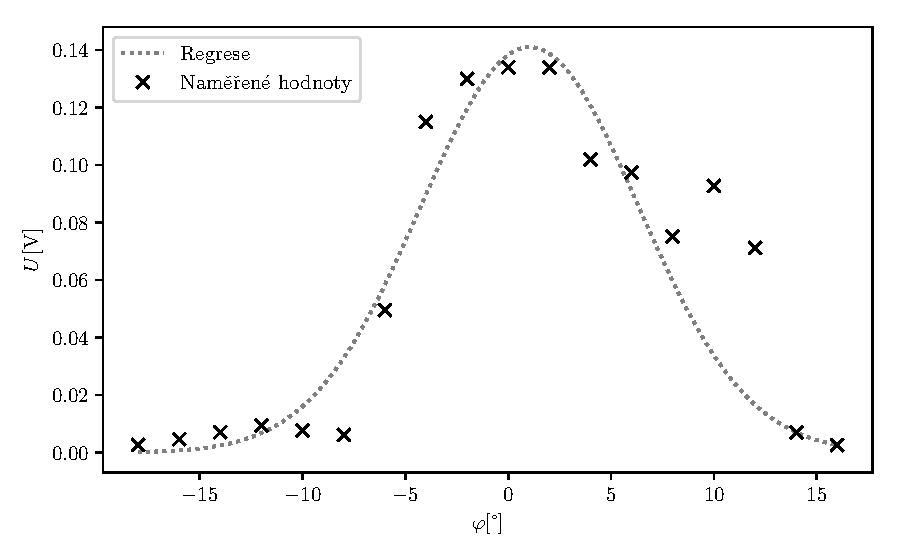
\includegraphics[]{apertura}
        \caption{Závislost napětí na fotodiodě na úhlu ramena aparatury}
        \label{fig:apertura}
      \end{figure}

  \section*{Diskuse}

  \section*{Závěr}
      
  \begin{thebibliography}{}
 
    \bibitem{pokyny}
    Pokyny k měření ``Vlnová optika'', dostupné z\\ \url{http://physics.mff.cuni.cz/vyuka/zfp/_media/zadani/pokyny/mereni_326.pdf}, 5.\,4.\,2018
   
  \end{thebibliography}

\end{document}